% !TeX root = ../../main.tex
\graphicspath{{Parts/2_Installation/graphics/}}
\subsection{\LaTeX{} installation}

The standard distribution of \LaTeX is TeX Live, which works on most platforms. Detailed instructions can be found \hyperlink{https://www.tug.org/texlive/}{here}. Windows users may download TeX Live from \url{https://www.tug.org/texlive/windows.html#install}, Mac users may do so using the MacTeX installer from \url{https://www.tug.org/mactex/mactex-download.html}, and Linux users can download TeX Live from \url{https://www.tug.org/texlive/quickinstall.html}. This is technically the only thing you need to install to start using \LaTeX{} locally, since all of these will also install a front end to edit your \LaTeX{} documents, as well as install most commonly used packages (I have never needed to manually install packages so far).

You can also use your preferred code editing front end to edit your \LaTeX{} code. I prefer using VSCode for this purpose, and recommend it due to its easy to use \LaTeX{} extension and abundance of other useful tools. I will cover this in the following subsection


\subsection{Using \LaTeX{} on VSCode}

The first step to this is obviously, downloading VSCode itself. You can do this at \url{https://code.visualstudio.com/download}. Once VSCode is downloaded, the LaTeX Workshop extension must be installed. This can be done by navigating to the Extensions tab on the sidebar and typing it into the search bar. This is shown below
\begin{figure}[ht!]
    \centering
    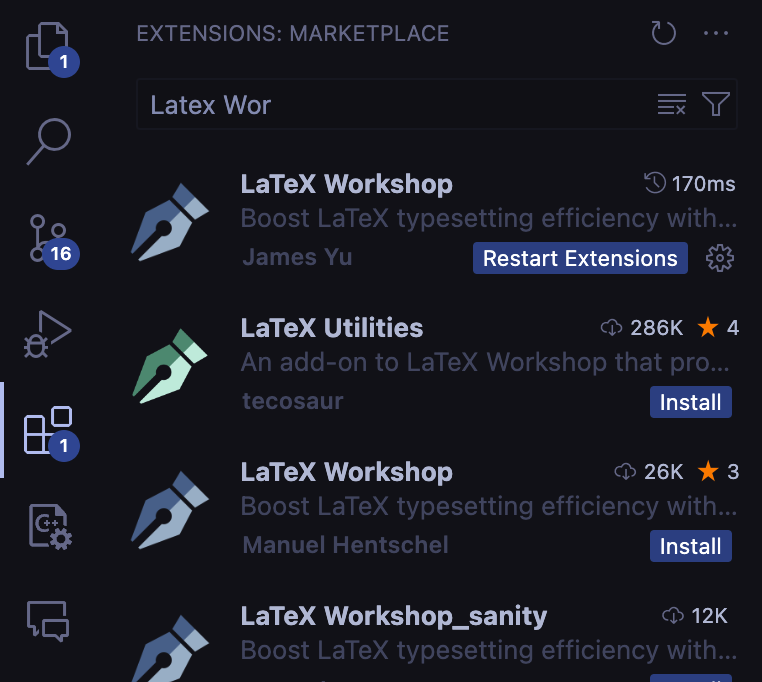
\includegraphics[width = 0.4\textwidth]{Extensions.png}
    \caption{The extension you want to install is the topmost one on the search results (the one by James Yu), which I have already installed in this image.}
\end{figure}

From here, you can simply create TeX files in VSCode by ending a file with the \verb|.tex| extension, and edit and compile them through the build button in the LaTeX Workshop sidebar tab, or the build button on top of the currently open TeX file. You can then use the LaTeX workshop sidebar once more to view the output PDF. Alternatively, you may find the output PDF in your file path and open it to the side in VSCode like you would a secondary tab of code. Nominally, this output PDF is in the same directory as your main TeX file. This is shown in \cref{fig:workspace}

\begin{figure}[ht!]
    \centering
    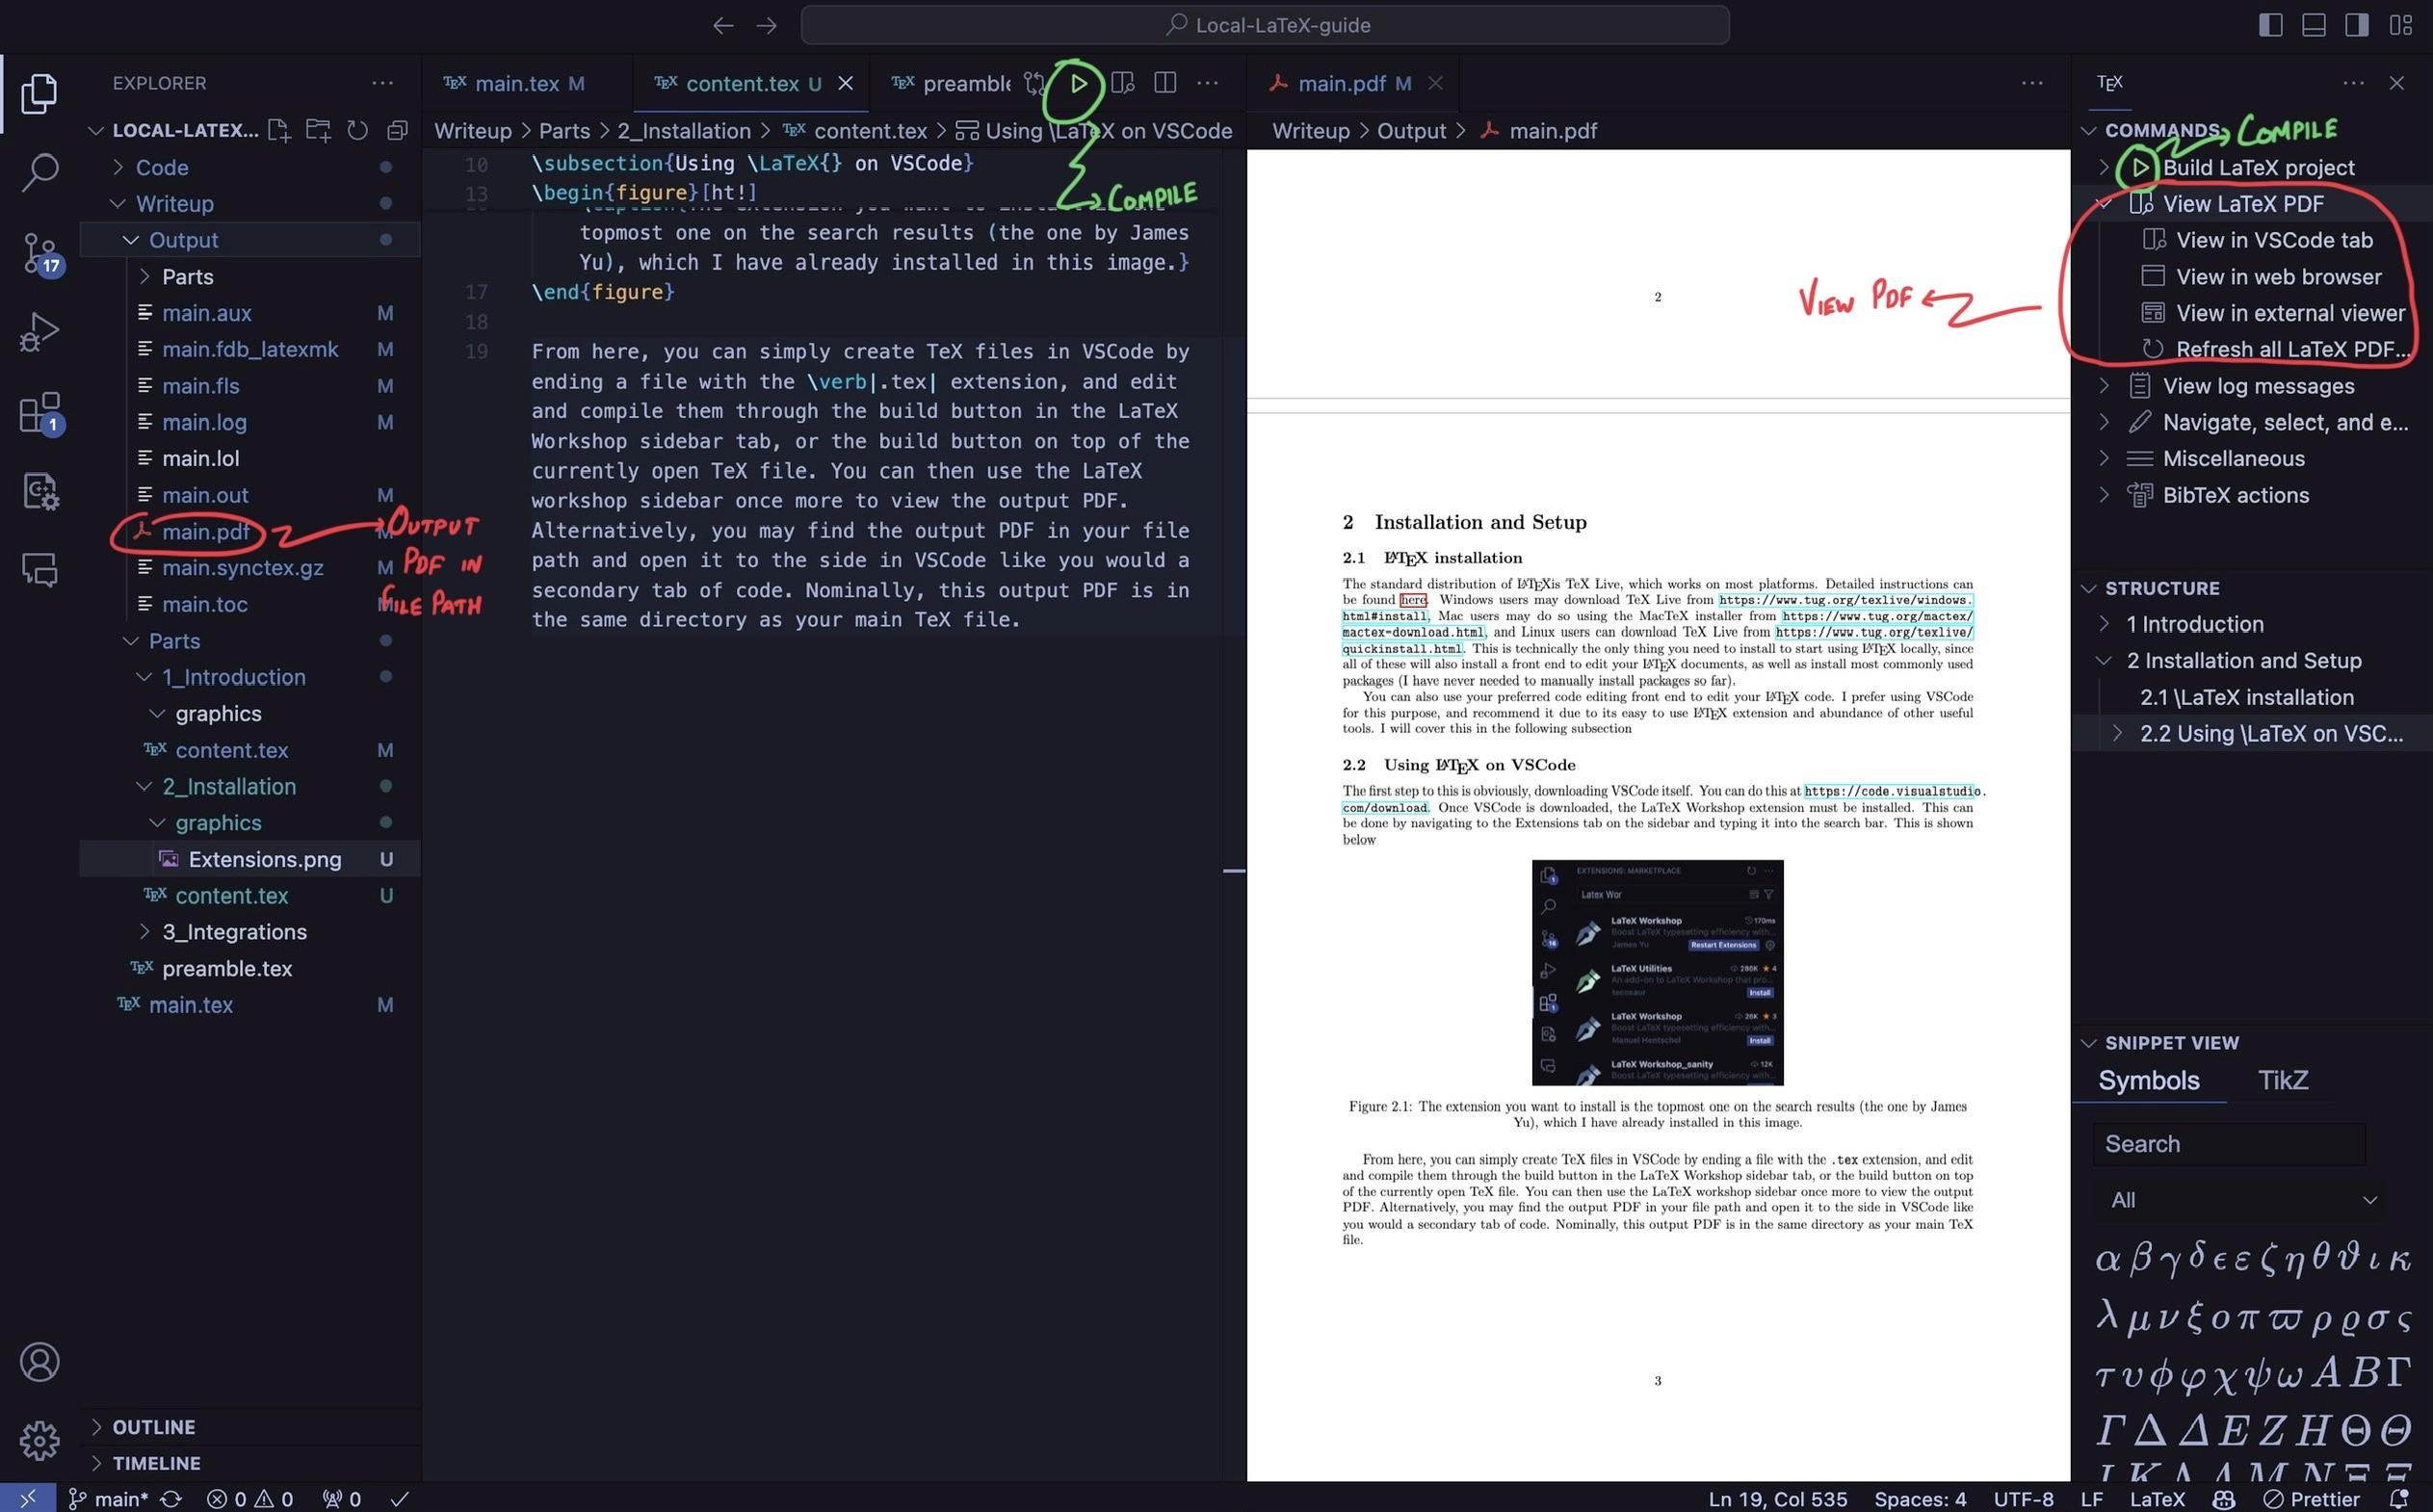
\includegraphics[width = \textwidth]{workspace.jpg}
    \caption{Where to find the output pdf and compile button in VSCode. Note that I moved the LaTeX workshop menu to the right sidebar in this picture, and have slightly modified the place where the output files go (more on this in a bit).}
    \label{fig:workspace}
\end{figure}